%------------------------------------------%
%			    Prima slide				   %
%        Caratterizzazione metropolis      %
%------------------------------------------%

\begin{frame}
    \frametitle{Caratterizzazione Metropolis}
    \framesubtitle{Modello XY}

    \begin{columns}
        \begin{column}{0.33\textwidth}
            \begin{block}{Termalizzazione}

                \begin{itemize}[itemsep=0.5em, label=$\diamond$]
                    \item $t_{t}$ maggiori per $T \to T_{KT}$
                    \item $t_{t}^{max}\,\simeq\,200$ sweeps
                \end{itemize}

                \vspace{0.5cm}

                \centering
                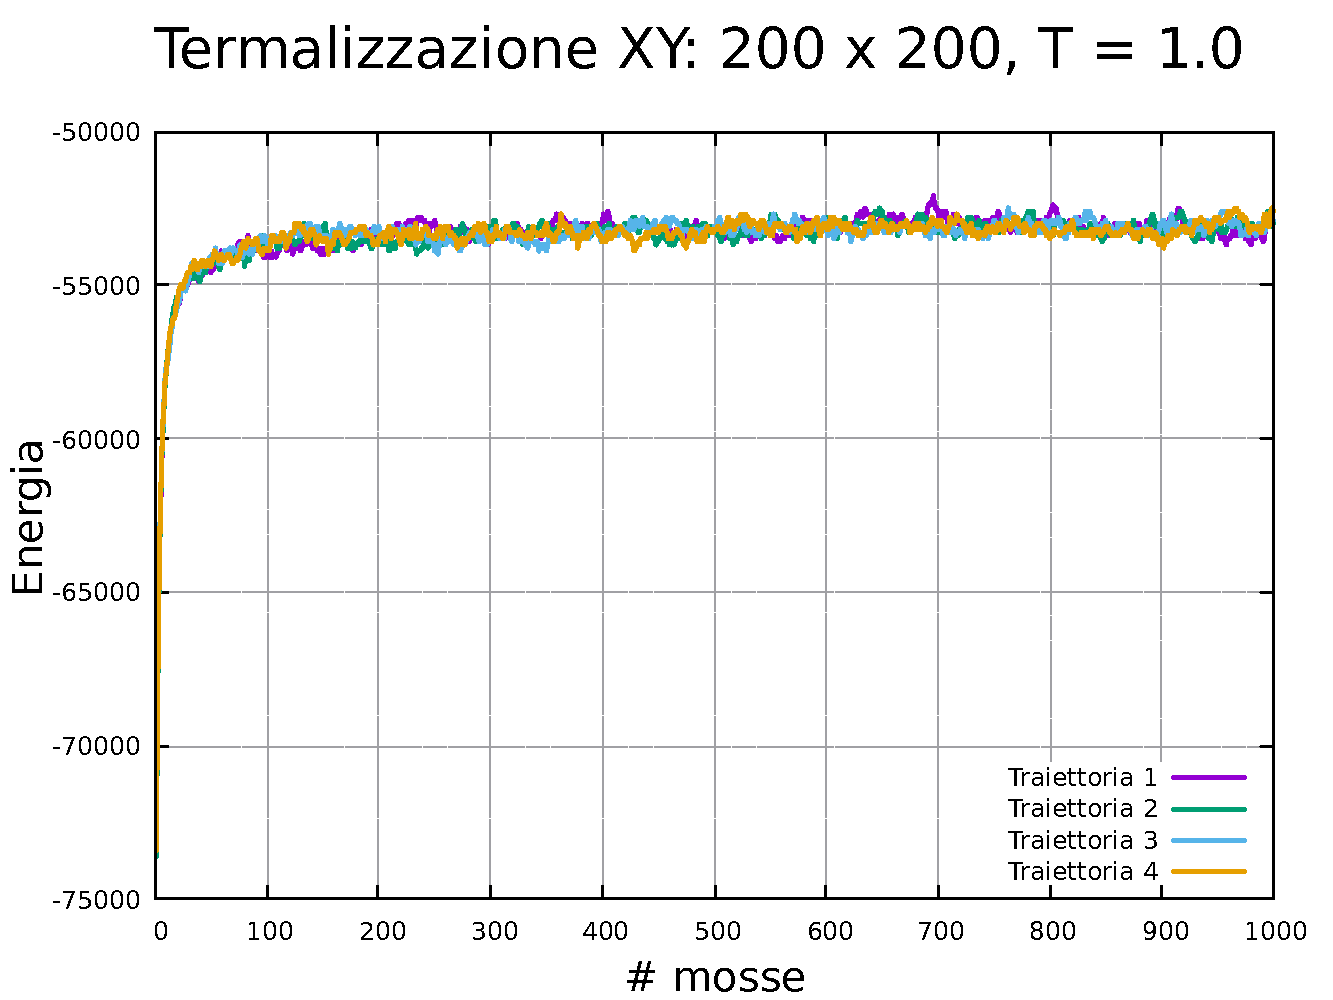
\includegraphics[width=\textwidth]{../ModelloXY/analisi/term/graphTerm/term_200_1.0.pdf}
            
            \end{block}
        \end{column}
    
        \begin{column}{0.33\textwidth}
            \begin{block}{Auto-correlazione}

                \begin{itemize}[itemsep=0.5em, label=$\diamond$]
                    \item $t_{c}$ maggiori per $T \to T_{KT}^-$
                    \item $t_{c}^{max}\,\simeq\,5000$ sweeps
                \end{itemize}

                \vspace{0.5cm}

                \centering
                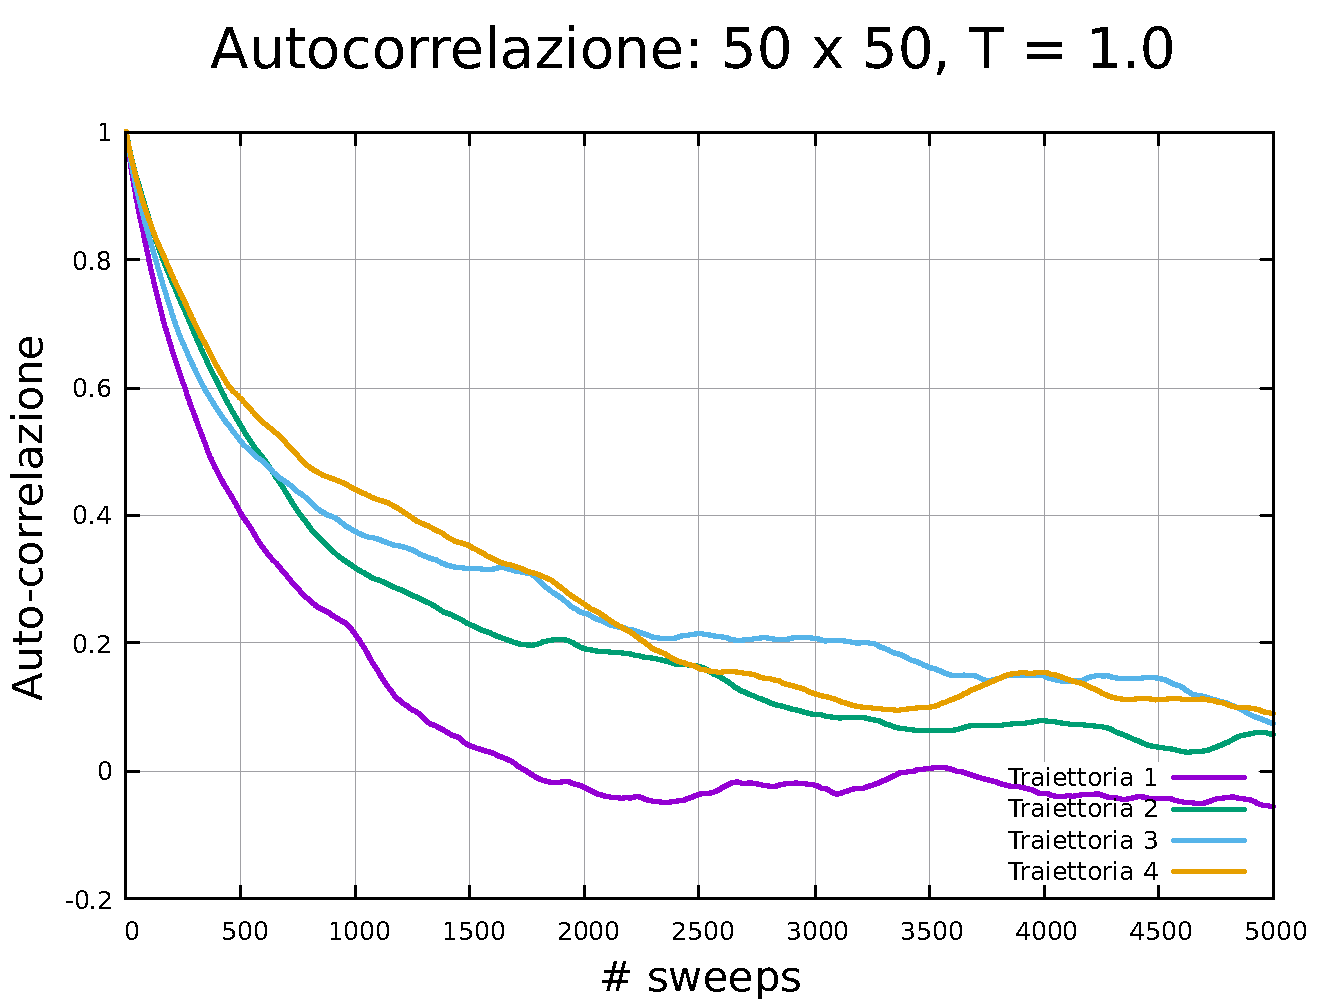
\includegraphics[width=\textwidth]{../ModelloXY/analisi/tcorr/auto/autoGraph/auto_50_1.0.pdf}

            \end{block}
        \end{column}

        \begin{column}{0.33\textwidth}
            \begin{block}{Blocchi}
                
                \begin{itemize}[itemsep=0.5em, label=$\diamond$]
                    \item $l_{b}$ maggiori per $T \to T_{KT}^-$
                    \item $l_{b}^{max}\,\simeq\,10000$ sweeps
                \end{itemize}

                \vspace{0.5cm}

                \centering
                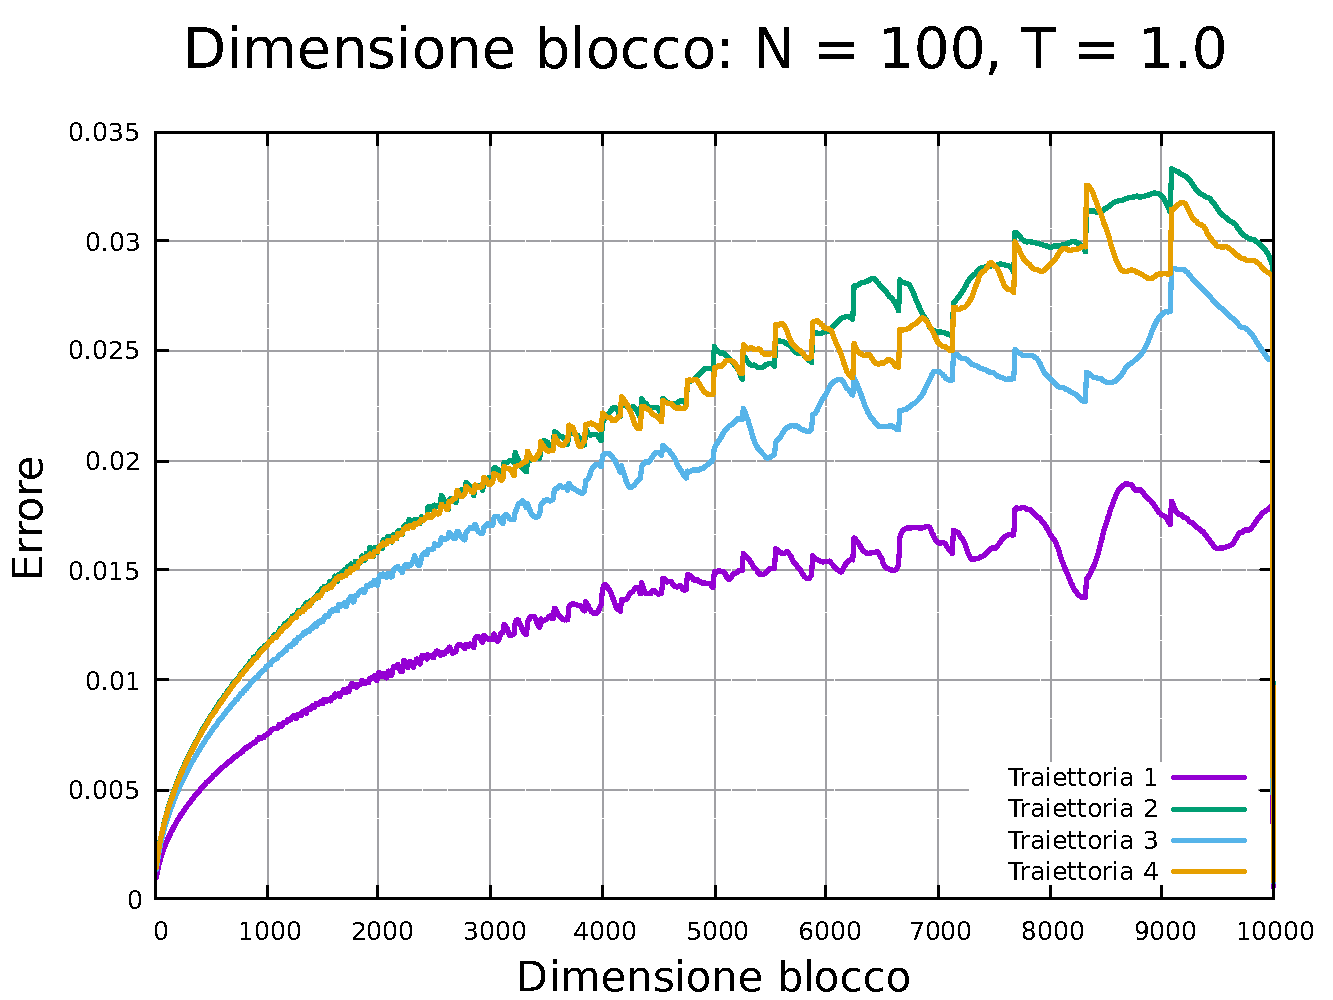
\includegraphics[width=\textwidth]{../ModelloXY/analisi/lblk/err/graphErr/lblk_100_1.0.pdf}

            \end{block}        
        \end{column}
    \end{columns}
\end{frame}



%-----------------------------------------%
%			  Seconda slide				  %
%	  Studio configurazioni low-highT  	  %
%-----------------------------------------%
\begin{frame}
    \frametitle{Configurazioni}
    \framesubtitle{ModelloXY}

    \begin{columns}
        \begin{column}{0.5\textwidth}
            \begin{block}{T = 0.5}

            \centering
            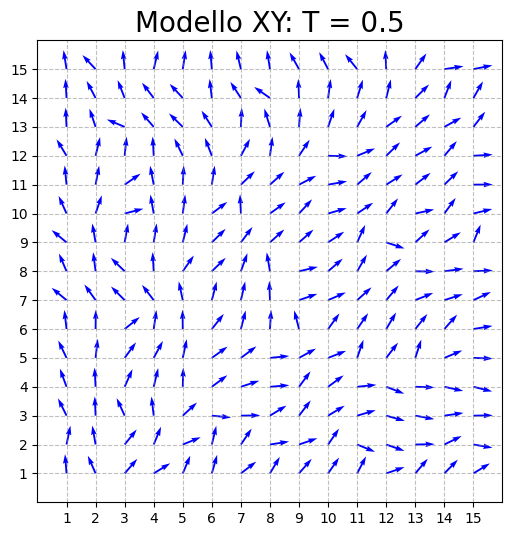
\includegraphics[width=0.8\textwidth]{Immagini/simXY/conf_T0.5.png}

            \end{block}
        \end{column}
    
        \begin{column}{0.5\textwidth}
            \begin{block}{T = 1.0}

                \centering
                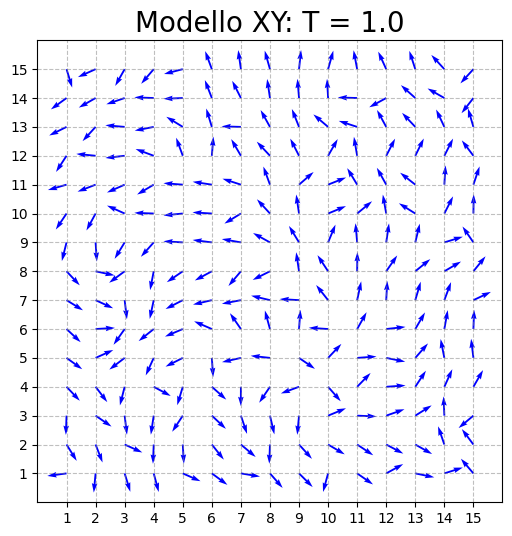
\includegraphics[width=0.8\textwidth]{Immagini/backupXY/conf_T1.0.png}

            \end{block}
        \end{column}
    \end{columns}

\end{frame}



%------------------------------------------%
%			    Terza slide	    		   %
%     Studio configurazioni a T mancanti   %
%------------------------------------------%
\begin{frame}
    \frametitle{Configurazioni}
    \framesubtitle{Modello XY}

    \begin{columns}
        \begin{column}{0.5\textwidth}
            \begin{block}{T = 1.5}

            \centering
            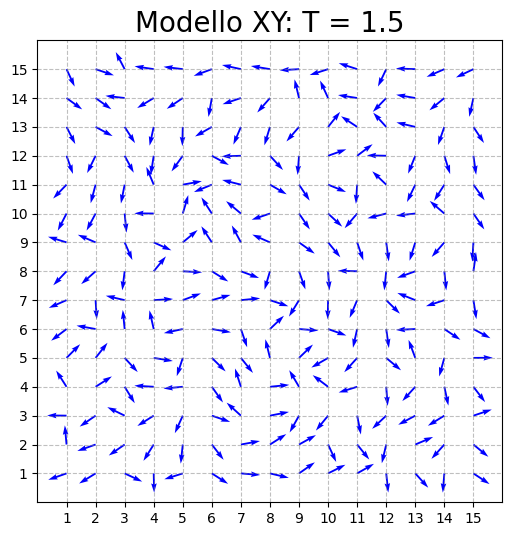
\includegraphics[width=0.8\textwidth]{Immagini/backupXY/conf_T1.5.png}

            \end{block}
        \end{column}
    
        \begin{column}{0.5\textwidth}
            \begin{block}{T = 2.0}

                \centering
                \includegraphics[width=0.8\textwidth]{Immagini/backupXY/conf_T2.0.png}

            \end{block}
        \end{column}
    \end{columns}

\end{frame}



%------------------------------------------%
%			    Quarta slide			   %
%     Studio configurazioni a T mancanti   %
%------------------------------------------%
\begin{frame}
    \frametitle{Configurazioni}
    \framesubtitle{Modello XY}

    \begin{columns}
        \begin{column}{0.5\textwidth}
            \begin{block}{T = 2.5}

            \centering
            \includegraphics[width=0.8\textwidth]{Immagini/simXY/conf_T2.5.png}

            \end{block}
        \end{column}
    
        \begin{column}{0.5\textwidth}
            \begin{block}{T = 3.0}

                \centering
                \includegraphics[width=0.8\textwidth]{Immagini/backupXY/conf_T3.0.png}

            \end{block}
        \end{column}
    \end{columns}

\end{frame}